% SVN Info:
% $Date: 2021-02-01 14:11:20 +0100 (Mo, 01 Feb 2021) $
% $Rev: 1041 $
% $Author: kolja $
The API is a DLL with C linkage.\par

The functions provided by the DLL are declared in \textsf{TimeTagger4\tu interface.h}.

\section{Constants}

	\crondef{TIMETAGGER4\tu CHANNEL\tu COUNT 4}\\
	The number of TDC input channels.\par

	\crondef{TIMETAGGER4\tu TIGER\tu COUNT 5}\\
	The number of timing generators. One for each TDC input and one for the Start input.\par

	\crondef{TIMETAGGER4\tu TRIGGER\tu COUNT 16}\\
	The number of potential trigger sources for the timing generators. One for each TDC input, one for the Start input plus some specials. 
	Not all triggeer sources are available on the \deviceName . See Section~\ref{cp:tigerblock} for details.\par

\section{Initialization}
		\cronvar{int}{timetagger4\tu close(}\cronvar{timetagger4\tu device}{*device)}\\
		Finalizes the driver for this device.

		\cronvar{int}{timetagger4\tu count\tu devices(}\cronvar{int}{*error\tu code}, \cronvar{char}{**error\tu message)}\\
		Returns the number of boards present in the system that are supported by this driver.\par

		\cronvar{int}{timetagger4\tu get\tu default\tu init\tu parameters(}\cronvar{timetagger4\tu init\tu parameters}{*init)}\\
		Sets up the standard parameters. Gets a set of default parameters for \textsf{timetagger4\tu init()}. This must always be used to initialize the \textsf{timetagger4\tu init\tu parameter()} structure.\par

		\cronvar{timetagger4\tu device}{*timetagger4\tu init(}\cronvar{timetagger4\tu init\tu parameters}{*params}, \\ \cronvar{int}{*error\tu code}, \cronvar{char}{**error\tu message)}\\
		Opens and initializes the \deviceName\ board with the given index. 
		With \textsf{error\tu code} and \textsf{error\tu message} the user must provide pointers to buffers where error information should be written by the driver.\par

		Params is a structure of type \textsf{timetagger4\tu init\tu parameters} that must be completely initialized.\par

		\subsection{Structure timetagger4\tu init\tu parameters}
			\cronvar{int}{version}\\
			The version number. Must be set to \textsf{TIMETAGGER4\tu API\tu VERSION}.\par

			\cronvar{int}{card\tu index}\\
			The index in the list of \deviceName\ boards that should be initialized.\\
			There might be multiple boards in the system that are handled by this driver as reported by \textsf{timetagger4\tu count\tu devices}. This index selects one of them. Boards are enumerated depending on the PCIe slot. 
			The lower the bus number and the lower the slot number the lower the card index.\par

			\cronvar{int}{board\tu id}\\
			the global index in all cronologic devices.\\
			This 8 bit number is filled into each packet created by the board and is useful if data streams of multiple boards will be merged. If only \deviceName\ cards are used this number can be set to the \textsf{card\tu index}. If boards of different types that use a compatible data format are used in a system each board should get a unique id.
			Can be changed with \textsf{int timetagger4\tu set\tu board\tu id\allowbreak(timetagger4\tu device *device, int board\tu id)}.\par

			\cronvar{\tu \tu int64}{buffer\tu size[8]}\\
			The minimum size of the DMA buffer.\\
			If set to 0 the default size of 16~MByte is used. For the \deviceName\ only the first entry is used.\par

			\cronvar{int}{buffer\tu type}\\
			The type of buffer. Must be set to 0.
			\begin{description}
				\item[] \crondef{TIMETAGGER4\tu BUFFER\tu ALLOCATE   0}
				\item[] \crondef{TIMETAGGER4\tu BUFFER\tu USE\tu PHYSICAL   1}  // unsupported
			\end{description}

			\cronvar{\tu \tu int64}{buffer\tu address}\\
			This is set by timetagger4\_init() to the start address of the reserved memory.\\ 
			The buffers will be allocated with the sizes given above. Make sure that the memory is large enough.\par

			\cronvar{int}{variant}\\
			Set to 0. Can be used to activate future device variants such as different base frequencies.\par

			\cronvar{int}{device\tu type}\\
			A constant for the different devices of cronologic \textsf{CRONO\tu DEVICE\tu *}.\\
			Initialized by \textsf{timetagger4\tu get\tu default\tu init\tu parameters()}. Must be left unchanged.
			\begin{itemize}
				\item[] \crondef{CRONO\tu DEVICE\tu HPTDC 1}
				\item[] \crondef{CRONO\tu DEVICE\tu NDIGO5G 2}
				\item[] \crondef{CRONO\tu DEVICE\tu NDIGO250M 4}
				\item[] \crondef{CRONO\tu DEVICE\tu xTDC4 6}
				\item[] \crondef{CRONO\tu DEVICE\tu TIMETAGGER4 8}
			\end{itemize}

			\cronvar{int}{dma\tu read\tu delay}\\
			The update delay of the write pointer after a packet has been sent over PCIe. Specified in multiples of 16ns
			Should not be changed by the user.\par

			\cronvar{int}{use\tu ext\tu clock}\\
			If set to 1 use external 10 MHz reference. If set to 0 use internal reference.\par

	\section{Status Information}
		\subsection{Functions for Information Retrieval}

			The driver provides functions to retrieve detailed information on the type of board, its configuration, settings and state. The information is split according to its scope and the computational requirements to query the information from the board.

			\cronvar{int}{timetagger4\tu get\tu driver\tu revision()}\\
			Returns the driver version, same format as timetagger4\tu static\tu info::driver\tu revision. This function does not require a \deviceName\ board to be present.

			\cronvar{const char*}{timetagger4\tu get\tu driver\tu revision\tu str()}\\
			Returns the driver version including SVN build revision as a string. This function does not require \deviceName\ board to be present.

			\cronvar{int}{timetagger4\tu get\tu fast\tu info(}\cronvar{timetagger4\tu device}{*device}, \cronvar{timetagger4\tu fast\tu info}{*info)}\\
			Returns fast dynamic information.\\
			This call gets a structure that contains dynamic information that can be obtained within a few microseconds.\par

			\cronvar{int}{timetagger4\tu get\tu param\tu info(}\cronvar{timetagger4\tu device}{*device}, \cronvar{timetagger4\tu param\tu info}{*info)}\\
			Returns configuration changes.\\
			Gets a structure that contains information that changes indirectly due to configuration changes.\par

			\cronvar{int}{timetagger4\tu get\tu slow\tu info(}\cronvar{timetagger4\tu device}{*device}, \cronvar{timetagger4\tu slow\tu info}{*info)}\\
			Returns slow dynamic information.\\
			The data reported in this structure requires milliseconds to be obtained. 
			The application should only call it in situations where the program flow can be blocked as long.\par

			\cronvar{int}{timetagger4\tu get\tu static\tu info(}\cronvar{timetagger4\tu device}{*device},\cronvar{timetagger4\tu static\tu info}{*info)}\\
			Contains static information.\\
			Gets a structure that contains information about the board that does not change during run time.\par

		\subsection{Structure timetagger4\tu static\tu info}

			This structure contains information about the board that does not change during run time. It is provided by the function \textsf{timetagger4\tu get\tu static\tu info}.\par

			\cronvar{int}{size}\\
			The number of bytes occupied by the structure.

			\cronvar{int}{version}\\
			A version number that is increased when the definition of the structure is changed. The increment can be larger than one to match driver version numbers or similar. Currently only version 0 is defined.\par


			\cronvar{int}{board\tu id}\\
			ID of the board.\\
			This value has been passed to the constructor by the user. It is reflected in the output data.\par

			\cronvar{int}{driver\tu revision}\\
			Encoded version number fo the driver.\\
			The lower three bytes contain a triple level hierarchy of version numbers, e.g. 0x010103 encodes version 1.1.3.\\
			A change in the first digit generally requires a recompilation of user applications. 
			Changes in the second digit denote significant improvements or changes that don't break compatibility 
			and the third digit increments with minor bug fixes and similar updates that do not affect the API.\par

			\cronvar{int}{firmware\tu revision}\\
			Revision number of the FPGA configuration.

			\cronvar{int}{board\tu revision}\\
			Board revision number.\\
			The board revision number can be read from a register. It is a four bit number that changes when the schematic of the board is changed.
			\begin{itemize}
				\item[0:] Experimental first board version. Labeled "Rev. 1"
				\item[1:] First commercial version. Labeled "Rev. 2"
				\item[2:] Updated commercial version. Labeled "Rev. 3"
				\item[4:] Lates commercial version. Labeled "Rev. 4"
			\end{itemize}

			\cronvar{int}{board\tu configuration}\\
			Describes the schematic configuration of the board.\\
			The same board schematic can be populated in multiple variants. This is a four bit code that can be read from a register.

			\cronvar{int}{subversion\tu revision}\\
			Subversion revision id of the FPGA configuration source code.

			\cronvar{int}{chip\tu id}\\
			\itett{
				Reserved.
				}{
				16 bit factory ID of the TDC chip.
				}\par

			\cronvar{int}{board\tu serial}\\
			Serial number.\\
			With year and running number in 8.24 format. The number is identical to the one printed on the silvery sticker on the board.\par

			\cronvar{unsigned int}{flash\tu serial\tu high}\\
			high 32 bits of 64 bit manufacturer serial number of the flash chip.

			\cronvar{unsigned int}{flash\tu serial\tu low}\\
			low 32 bits of 64 bit manufacturer serial number of the flash chip

			\cronvar{int}{flash\tu valid}\\
			If not 0 the driver found valid calibration data in the flash on the board and is using it.\par

		\subsection{Structure timetagger4\tu param\tu info}
			This struct contains configuration changes provided by timetagger4\tu get\tu param\tu info().

			\cronvar{int}{size}\\
			The number of bytes occupied by the structure. \par

			\cronvar{int}{version}\\
			A version number that is increased when the definition of the structure is changed. The increment can be larger than one to match driver version numbers or similar. Currently only version 0 is defined.\par


			\cronvar{double}{binsize}
			Bin size (in ps) of the measured TDC data.

			\cronvar{int}{board\tu id}\\
			Board ID.\\
			The board uses this ID to identify itself in the output data stream. The ID takes values between 0 and 255.\par

			\cronvar{int}{channels}\\
			Number of channels of the board.\\
			Returns 4.\par

			\cronvar{int}{channel\tu mask}\\
			Bit assignment of each enabled input channel.\\
			Bit $n <= 0 < 4$ is set if channel n is enabled. \par

			\cronvar{\tu\tu int64}{total\tu buffer}\\
			The total amount of DMA buffer in bytes.

		\subsection{Structure timetagger4\tu fast\tu info}

			\cronvar{int}{size}\\
			The number of bytes occupied by the structure. \par

			\cronvar{int}{version}\\
			A version number that is increased when the definition of the structure is changed. The increment can be larger than one to match driver version numbers or similar. Currently only version 0 is defined.\par


			\cronvar{int}{tdc\tu rpm}\\
			Speed of the TDC fan in rounds per minute. Reports 0 if no fan is present.\par

			\cronvar{int}{fpga\tu rpm}\\
			Speed of the FPGA fan in rounds per minute. Reports 0 if no fan is present.\par

			\cronvar{int}{alerts}\\
			Alert bits from temperature sensor and the system monitor.
			\itett{
				The TimeTagger4 does not implement any temperature alerts.
			}{
				Bit 0 is set if the TDC temperature exceeds 140°C. The TDC did shut down and the device needs to be reinitialized. 
			}\par

			\cronvar{int}{pcie\tu pwr\tu mgmt}\par
			Allways 0. 

			\cronvar{int}{pcie\tu link\tu width}\\
			Number of PCIe lanes the card uses. Should always be 1 for the \deviceName. \par

			\cronvar{int}{pcie\tu max\tu payload}\\
			Maximum size in bytes for one PCIe transaction. Depends on system configuration.\par

	\section{Configuration}

		The device is configured with a configuration structure. 
		The user should first obtain a structure that contains the default settings of the device read from an on board ROM , 
		then modify the structure as needed for the user application and use the result to configure the device.\par

		\cronvar{int}{timetagger4\tu configure(}\cronvar{timetagger4\tu device} {*device,} \\ \cronvar{timetagger4\tu configuration}{*config)}\\
		Configures the \deviceName\ device.\par

		\cronvar{int}{timetagger4\tu get\tu current\tu configuration(}\cronvar{timetagger4\tu device}{*device,} \\ \cronvar{timetagger4\tu configuration}{*config)}\\
		Gets current configuration. Copies the current configuration to the specified config pointer.\par

		\cronvar{int}{timetagger4\tu get\tu default\tu configuration(}\cronvar{timetagger4\tu device}{*device,} \\ \cronvar{timetagger4\tu configuration}{*config)}\\
		Gets default configuration. Copies the default configuration to the specified config pointer.\par

		\subsection{Structure timetagger4\tu configuration}

			This is the structure containing the configuration information. It is used in conjunction with \textsf{timetagger4\tu get\tu default\tu configuration()}, \textsf{timetagger4\tu get\tu current\tu configuration()} and \textsf{timetagger4\tu configure()}.\par

			It uses the substructures \textsf{timetagger4\tu tiger\tu block} and \textsf{timetagger4\tu trigger}.\par

			\cronvar{int}{size}\\
			The number of bytes occupied by the structure.\par

			\cronvar{int}{version}\\
			A version number that is increased when the definition of the structure is changed. The increment can be larger than one to match driver version numbers or similar. Currently only version 0 is defined.\par

			\cronvar{int}{tdc\tu mode}\\
			TDC mode. Can be grouped or continuous. \\
			Currently only TIMETAGGER4\tu TDC\tu MODE\tu GROUPED is supported. 
			This is set per default by timetagger4\tu get\tu current\tu configuration() and should be left unchanged.\par

			\cronvar{crono\tu bool\tu t}{start\tu rising} 
			\itett{
				Not applicable for the \deviceName.
			}{
				Selects whether the rising or falling edge of the start signal is used to start a group.
			}\par

			\cronvar{double}{dc\tu offset[TIMETAGGER4\tu CHANNEL\tu COUNT + 1]}\\
			Set the threshold voltage for the input channels S, A - D (see figure \ref{fig:dcoffset1}).
			\begin{itemize}
				\item dc\tu offset[0] : threshold for channel Start
				\item dc\tu offset[1 - 4] : threshold for channels A \ldots D
			\end{itemize}
			Supported range is -1.32V to +1.18V. This should be close to 50\% of the height of the input pulse. Examples for various signaling standards are defined as follows\par
			\begin{tabular}{ll}
				\crondef{DC\tu OFFSET\tu P\tu NIM} & +0.35\\
				\crondef{DC\tu OFFSET\tu P\tu CMOS} & +1.18\\
				\crondef{DC\tu OFFSET\tu P\tu LVCMOS\tu 33} & +1.18\\
				\crondef{DC\tu OFFSET\tu P\tu LVCMOS\tu 25} & +1.18\\
				\crondef{DC\tu OFFSET\tu P\tu LVCMOS\tu 18} & +0.90\\
				\crondef{DC\tu OFFSET\tu P\tu TTL} & +1.18\\
				\crondef{DC\tu OFFSET\tu P\tu LVTTL\tu 33} & +1.18\\
				\crondef{DC\tu OFFSET\tu P\tu LVTTL\tu 25} & +1.18\\
				\crondef{DC\tu OFFSET\tu P\tu SSTL\tu 3} & +1.18\\
				\crondef{DC\tu OFFSET\tu P\tu SSTL\tu 2} & +1.18\\
				\crondef{DC\tu OFFSET\tu N\tu NIM} & -0.35\\
				\crondef{DC\tu OFFSET\tu N\tu CMOS} & -1.32\\
				\crondef{DC\tu OFFSET\tu N\tu LVCMOS\tu 33} & -1.32\\
				\crondef{DC\tu OFFSET\tu N\tu LVCMOS\tu 25} & -1.25\\
				\crondef{DC\tu OFFSET\tu N\tu LVCMOS\tu 18} & -0.90\\
				\crondef{DC\tu OFFSET\tu N\tu TTL} & -1.32\\
				\crondef{DC\tu OFFSET\tu N\tu LVTTL\tu 33} & -1.32\\
				\crondef{DC\tu OFFSET\tu N\tu LVTTL\tu 25} & -1.25\\
				\crondef{DC\tu OFFSET\tu N\tu SSTL\tu 3} & -1.32\\
				\crondef{DC\tu OFFSET\tu N\tu SSTL\tu 2} & -1.25\\
			\end{tabular}\par
			 \noindent The inputs are AC coupled. Thus, the absolute voltage is not important for pulse inputs. It is the relative pulse amplitude that causes the input circuits to switch. \textit{dc\tu offset} must be set to the relative switching voltage for the input standard in use. If the pulses are negative, a negative switching threshold must be set and vice versa.
			\begin{figure}
				\begin{center}
					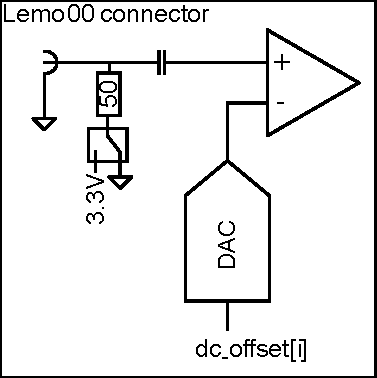
\includegraphics[width=0.3\textwidth]{figures/InputCircuit.pdf}
					\caption{Input circuit for each of the five input channels. Both inputs of the buffer are biased at 1.32V by default.\label{fig:dcoffset1}}
				\end{center}
			\end{figure}
%%			\begin{figure}
%%				\begin{center}
%%					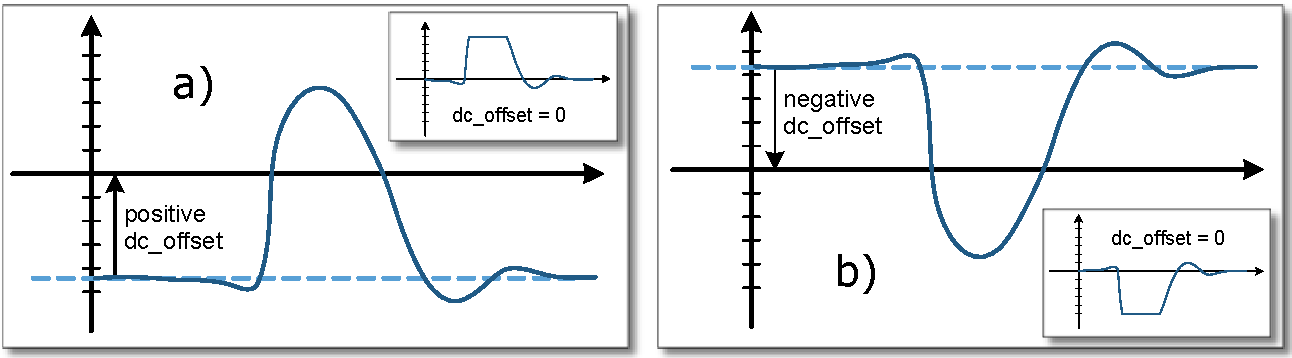
\includegraphics[width=\textwidth]{figures/dc_offset.pdf}
%%%					\caption{\textit{dc\tu offset} is used to shift the signal on each input channel such that the noise margin relative to the switching threshold is maximized.
%%					Insets of figure a) and b) show the base line of the signal with $\mathrm{\textit{dc\tu offset}}~=~0$ close to the switching threshold of the input buffer. Figure a) shows the positive pulse with $\mathrm{\textit{dc\tu offset}}~>~0$ and figure b) shows the negative pulse with $\mathrm{\textit{dc\tu offset}}~<~0$.\label{fig:dcoffset2}}
%%				\end{center}
%%			\end{figure}

			\cronvar{timetagger4\tu trigger}{trigger[TIMETAGGER4\tu TRIGGER\tu COUNT]}\\
			Configuration the polarity of the external trigger sources.
			These are used as inputs for the TiGer blocks and as inputs to the time measurement unit.\par

			\cronvar{timetagger4\tu tiger\tu block}{tiger\tu block[TIMETAGGER4\tu TIGER\tu COUNT]}
			Configuration of the timing generator (TiGeR).

			\cronvar{timetagger4\tu channel}{channel[TIMETAGGER4\tu CHANNEL\tu COUNT]}\\
				Configure the TDC channels.

			\cronvar{timetagger4\tu lowres\tu channel}{lowres\tu channel[TIMETAGGER4\tu LOWRES\tu CHANNEL\tu COUNT]}\\
			\itett{
				Not applicable for \deviceName. 
			}{
				Only applicable to the xTDC4-Sciex. Configures the additional digital lowres inputs.
			}\par

			\cronvar{int}{auto\tu trigger\tu period}\\
			\cronvar{int}{auto\tu trigger\tu random\tu exponent}\\
			Create a trigger either periodically or randomly. There are two parameters $M = \text{trigger\tu period}$ and $N = \text{random\tu exponent}$ that result in a distance between triggers of $T$ clock cycles.

			\begin{align}
				T &= 1 + M + [1...2^N]\\
				&0 \leq M < 2^{32}\\
				&0 \leq N < 32
			\end{align}

			\noindent There is no enable or reset as the usage of this trigger can be configured in the TiGer block channel source field.\par

			\subsection{Structure timetagger4\tu trigger}
			\label{structtrigger}
			\cronvar{crono\tu bool\tu t}{falling}\\
			\cronvar{crono\tu bool\tu t}{rising}\\
			Select for which edges a trigger event is created inside the FPGA.
			\itett{
				The \deviceName can output measurements for one or both edges of input signals. 
			}{
				The \deviceName can output measurements with a reduced bin size of $5/6~ns = 833,\overline{3}~ps$ for one or both edges of input signals. 
				See section \ref{difficulthits} for more information on hits with varying resolution.
				Use \textsf{xtdc4\tu channel.rising} on page \pageref{structchannel} to select which edge is measured with full resolution.
				The edge that is selected for full resolution measurement must also be enabled for low resolution measurement.
			}\par

			\subsection{Structure timetagger4\tu tiger\tu block\label{cp:tigerblock}}

			\cronvar{crono\tu bool\tu t}{enable}\\
			Activates the timing generator (TiGer).\par
	
			\cronvar{crono\tu bool\tu t}{negate}\\
			Inverts output polarity. Default is set to false.\par
	
			\cronvar{crono\tu bool\tu t}{retrigger}\\
			Enables retrigger setting.\\
			If enabled the timer is reset to the value of the \textsf{start} parameter, whenever the input signal is set while waiting to reach the \textsf{stop} time.\par
	
			\cronvar{crono\tu bool\tu t}{extend}\\
			Not implemented.
	
			\cronvar{crono\tu bool\tu t}{enable\tu lemo\tu output}\\
			Enables the LEMO output. Drive the TiGer Signal to the corresponding Lemo connector as an output. 
			This is DC coupled, so make sure that you do not any devices connected as inputs.
			Pulses created by the TiGer are visible at the \deviceName inputs and can be measured again to get the exact timing.  
	
			\cronvar{int}{start}\\
			\cronvar{int}{stop}\\
			\itett{
				In multiples of $4~ns$.
			}{
				In multiples of $20/3 = 6,\overline{6}~ns$
			}
			The time during which the TiGer output is set, relativ to the trigger input. The parameters \textsf{start} and \textsf{stop} must fulfill the following conditions:
			\[ 0 <= start <= stop <= 2^{16}-1 \]
			If retriggering is enabled, the timer is reset to the value of the start parameter whenever the input signal is set while waiting for the stop time. \par
			
	
			\cronvar{int}{sources}\\
			A bit mask with a bit set for all trigger sources that can trigger this TiGer block. 
			Default is \textsf{TIMETAGGER4\tu TRIGGER\tu SOURCE\tu S}.\par
	
			\begin{tabular}{lc}
					\crondef{TIMETAGGER4\tu TRIGGER\tu SOURCE\tu S} & 0x00000001\\
					\crondef{TIMETAGGER4\tu TRIGGER\tu SOURCE\tu A} & 0x00000002\\
					\crondef{TIMETAGGER4\tu TRIGGER\tu SOURCE\tu B} & 0x00000004\\
					\crondef{TIMETAGGER4\tu TRIGGER\tu SOURCE\tu C} & 0x00000008\\
					\crondef{TIMETAGGER4\tu TRIGGER\tu SOURCE\tu D} & 0x00000010\\
					%\crondef{TIMETAGGER4\tu TRIGGER\tu SOURCE\tu S1} & 0x00000020\\
					%\crondef{TIMETAGGER4\tu TRIGGER\tu SOURCE\tu S2} & 0x00000040\\
					%\crondef{TIMETAGGER4\tu TRIGGER\tu SOURCE\tu GATE} & 0x00000080\\
					\crondef{TIMETAGGER4\tu TRIGGER\tu SOURCE\tu AUTO} & 0x00004000\\
					\crondef{TIMETAGGER4\tu TRIGGER\tu SOURCE\tu ONE} & 0x00008000
				\end{tabular} 
	
			\subsection{Structure timetagger4\tu channel}
				\label{structchannel}
				Contains TDC channel settings.\par
	
				\cronvar{crono\tu bool\tu t}{enabled}\\
				Enable TDC channel.\par
	
				\cronvar{crono\tu bool\tu t}{rising}\\
				\itett{
					Not applicable for \deviceName.
				}{
					Select which edge of the signal is used for full resolution measurements. 
					\textsf{xtdc4\tu trigger.rising} and \textsf{xtdc4\tu trigger.falling} described on page \pageref{structtrigger} are used 
					to select which edges are recorded for low resolution measurement. 
					The edge that is selected for full resolution measurement must also be enabled for low resolution measurement.
					See section \ref{difficulthits} for more information on hits with varying resolution.
				}\par

				\itett{}{ % onyl for xTDC4
					\cronvar{crono\tu bool\tu t}{cc\tu enable}\\
					Enable carry chain TDC. This is set to \emph{true} by default an should be left unchanged. \par
	
					\cronvar{crono\tu bool\tu t}{cc\tu same\tu edge}\\
					Sets whether the carry chain TDC records the same or opposite edge as the TDC chip. 
					If the same edge is selected, that carry chain TDC acts  as a backup if the chip misses hits due to FIFO overflows or short input pulses.
					If opposite edges are selected, both edges of a pulse can be measured with reasonable resolution. See section \ref{difficulthits} for more information.\par
	
					\cronvar{crono\tu bool\tu t}{ths788\tu disable}\\
					Disable full resolution timestamps. This is set to \emph{false} by default and should be left unchanged.\par
				}
	
				\cronvar{int}{start}\\
				\cronvar{int}{stop}\\
				Veto function for grouping of hits into packets in multiples of the binsize. Only hits between start and stop are read out.
				The parameters must adhere to the following relations:
				\[
					0 <= start <= stop < 2^{ \itett{31}{30}}
				\]
	
	
		\section{Run Time Control}
	
				\cronvar{int}{timetagger4\tu continue\tu capture(}\cronvar{timetagger4\tu device}{*device)}\\
				Call this to resume data acquisition after a call to \textsf{timetagger4\tu pause\tu capture()}.\par
	
				\cronvar{int}{timetagger4\tu pause\tu capture(}\cronvar{timetagger4\tu device}{*device)}\\
				Pause data acquisition.\par
	
				\cronvar{int}{timetagger4\tu start\tu capture(}\cronvar{timetagger4\tu device}{*device)}\\
				Start data acquisition.\par
	
				\cronvar{int}{timetagger4\tu start\tu tiger(\cronvar{timetagger4\tu device}{*device})}\\
				Start timing generator.\par
	
				\cronvar{int}{timetagger4\tu stop\tu capture(}\cronvar{timetagger4\tu device}{*device)}\\
				Stop data acquisition.\par
	
				\cronvar{int}{timetagger4\tu stop\tu tiger(\cronvar{timetagger4\tu device}{*device})}\\
				Stop timing generator.\par
	
		\section{Readout\label{cp:readout}}
	
			\cronvar{int}{timetagger4\tu acknowledge(}\cronvar{timetagger4\tu device}{*device,} \cronvar{crono\tu packet}{*packet)}\\
			Acknowledges the processing of the last read block. This is only necessary if \textsf{timetagger4\tu read()} is not called with 
			\textsf{in.acknowledge\tu last\tu read} set.\\
			This feature allows to either free up partial DMA space early if there will be no call to \textsf{timetagger4\tu read} anytime soon. 
			It also allows to keep data over multiple calls to \textsf{timetagger4\tu read} to avoid unnecessary copying of data. \par
	
			\cronvar{int}{timetagger4\tu get\tu device\tu type}\\
			Returns the type of the device.	\textsf{CRONO\tu DEVICE\tu TIMETAGGER4}\par
	
			\cronvar{const char*}{timetagger4\tu get\tu last\tu error\tu message(\cronvar{timetagger4\tu device}{*device})}\\
			Returns most recent error message.\par
	
			\cronvar{int}{timetagger4\tu read(}\cronvar{timetagger4\tu device}{*device,} \cronvar{timetagger4\tu read\tu in}{*in,} \\ \cronvar{timetagger4\tu read\tu out}{*out)}\\
			Return a pointer to an array of captured data in \textsf{read\tu out}. 
			The result can contain any number of packets of type \textsf{timetagger4\tu packet}.
			\textsf{read\tu in} provides parameters to the driver. 
			A call to this method automatically allows the driver to reuse the memory returned in the previous call if \textsf{read\tu in.acknowledge\tu last\tu read} is set.\\
			Returns an error code as defined in the structure \textsf{timetagger4\tu read\tu out}.
	
			\subsection{Input Structure timetagger4\tu read\tu in}
	
				\cronvar{timetagger4\tu bool\tu t}{acknowledge\tu last\tu read}\\
				If set \textsf{timetagger4\tu read()} automatically acknowledges packets from the last read.
	
			\subsection{Input Structure timetagger4\tu read\tu out}
				\cronvar{crono\tu packet}{*first\tu packet}\\
				Pointer to the first packet that was capture by the call of \textsf{timetagger4\tu read}.\par
	
				\cronvar{crono\tu packet}{*last\tu packet}\\
				Address of header of the last packet in the buffer.\par
	
				\cronvar{int}{error\tu code}\\
				Assignments of the error codes.\par
				\begin{tabular}{lc}
					\crondef{CRONO\tu READ\tu OK} & 0\\
					\crondef{CRONO\tu READ\tu NO\tu DATA} & 1\\
					\crondef{CRONO\tu READ\tu INTERNAL\tu ERROR} & 2\\
					\crondef{CRONO\tu READ\tu TIMEOUT} & 3\par
				\end{tabular}\par
	
				\cronvar{const char}{*error\tu message}
				The last error in human readable form, possibly with additional information on the error.